% -*- coding: utf-8; -*-
% vim: set fileencoding=utf-8 :
\documentclass[english,submission]{programming}
%% First parameter: the language is 'english'.
%% Second parameter: use 'submission' for initial submission, remove it for camera-ready (see 5.1)


%
% Packages and Commands specific to article (see 3)
%
% These ones  are used in the guide, replace with your own.
%
\usepackage{multicol}
\usepackage{ccicons}
\usepackage{enumitem}
\setlist[itemize]{itemsep=0.5em}

\lstdefinelanguage[programming]{TeX}[AlLaTeX]{TeX}{%
  deletetexcs={title,author,bibliography},%
  deletekeywords={tabular},
  morekeywords={abstract},%
  moretexcs={chapter},%
  moretexcs=[2]{title,author,subtitle,keywords,maketitle,titlerunning,authorinfo,affiliation,authorrunning,paperdetails,acks,email},
  moretexcs=[3]{addbibresource,printbibliography,bibliography},%
}%
\lstset{%
  language={[programming]TeX},%
  keywordstyle=\firamedium,
  stringstyle=\color{RosyBrown},%
  texcsstyle=*{\color{Purple}\mdseries},%
  texcsstyle=*[2]{\color{Blue1}},%
  texcsstyle=*[3]{\color{ForestGreen}},%
  commentstyle={\color{FireBrick}},%
  escapechar=`,}
\newcommand*{\CTAN}[1]{\href{http://ctan.org/tex-archive/#1}{\nolinkurl{CTAN:#1}}}
%%


%%%%%%%%%%%%%%%%%%
%% These data MUST be filled for your submission. (see 5.3)
\paperdetails{
  %% perspective options are: art, sciencetheoretical, scienceempirical, engineering.
  %% Choose exactly the one that best describes this work. (see 2.1)
  perspective=engineering,
  %% State one or more areas, separated by a comma. (see 2.2)
  %% Please see list of areas in http://programming-journal.org/cfp/
  %% The list is open-ended, so use other areas if yours is/are not listed.
  area={Programming Systems},
  %% You may choose the license for your paper (see 3.)
  %% License options include: cc-by (default), cc-by-nc
  % license=cc-by,
}
%%%%%%%%%%%%%%%%%%

%%%%%%%%%%%%%%%%%%
%% These data are provided by the editors. May be left out on submission.
%\paperdetails{
%  submitted=2016-08-10,
%  published=2016-10-11,
%  year=2016,
%  volume=1,
%  issue=1,
%  articlenumber=1,
%}
%%%%%%%%%%%%%%%%%%


\begin{document}

\title{Design Choices of Document-Oriented Programming Systems}
%\subtitle{Preparing Articles for Programming}% optional
%\titlerunning{Preparing Articles for Programming} %optional, in case that the title is too long; the running title should fit into the top page column

\author[a]{Tomas Petricek}[0000-0002-7242-2208]
\authorinfo{is an assistant professor at Charles University. He
is interested in finding easier and more accessible ways of thinking
about programming. To do so, he combines technical work on
programming systems and tools with research into history and
philosophy of science. His work can be found at \href{https://tomasp.net}{\texttt{tomasp.net}} and
he can be reached at \email{tomas@tomasp.net}.}
\affiliation[a]{Charles University, Prague, Czechia}

\author[b]{Jonathan Edwards}[0000-0003-1958-7967]
\authorinfo{is an independent researcher working on drastically simplifying programming. He is known
for his Subtext series of programming language experiments and his blog at \href{https://alarmingdevelopment.org}{\texttt{alarmingdevelopment.org}}.
He has been a researcher at MIT CSAIL and CDG/HARC. He tweets \href{https://x.com/jonathoda}{\texttt{@jonathoda}} and can be reached at
\email{jonathanmedwards@gmail.com}.}
\affiliation[b]{Independent, Boston, MA, USA}

\author[a]{Joel Jakubovic}[0000-0003-0252-9066]
\authorinfo{todo}


% \authorrunning{T. Pape, C. Lopes, R. Hirschfeld} % Optional, for long author lists

%\keywords{programming journal, paper formatting, submission preparation} % please provide 1--5 keywords


%%%%%%%%%%%%%%%%%%%%%%%%%%%%%
% Please go to https://dl.acm.org/ccs/ccs.cfm and generate your Classification
% System [view CCS TeX Code] stanz and copy _all of it_ to this place.
%% From HERE
%\begin{CCSXML}
%<ccs2012>
%<concept>
%<concept_id>10002944.10011122.10003459</concept_id>
%<concept_desc>General and reference~Computing standards, RFCs and guidelines</concept_desc>
%<concept_significance>300</concept_significance>
%</concept>
%<concept>
%<concept_id>10010405.10010476.10010477</concept_id>
%<concept_desc>Applied computing~Publishing</concept_desc>
%<concept_significance>300</concept_significance>
%</concept>
%</ccs2012>
%\end{CCSXML}
%
%\ccsdesc[300]{General and reference~Computing standards, RFCs and guidelines}
%\ccsdesc[500]{Applied computing~Publishing}

% To HERE
%%%%%%%%%%%%%%%%%%%%%%%

\maketitle

% Please always include the abstract.
% The abstract MUST be written according to the directives stated in
% http://programming-journal.org/submission/
% Failure to adhere to the abstract directives may result in the paper
% being returned to the authors.
\begin{abstract}

% Context: What is the broad context of the work? What is the importance of the general research area?
Many interesting programming systems treat programming as document manipulation.
Examples include spreadsheets, data science notebooks, educational environments like Boxer and
multiple recent research programming systems. In such systems, the programmer interacts with a
document that contains a structured representation of both code and data, they modify the code
and data, trigger computations and view the results from the unified document interface.
%
% Inquiry: What problem or question does the paper address? How has this problem or question been addressed by others (if at all)?
Those \emph{document-oriented programming systems} have a unique set of design choices. The
concepts that we need to understand them and design them differ from the well-understood design
choices known from programming languages and other programming systems.

% Approach: What was done that unveiled new knowledge?
The aim of this paper is to identify the key design choices that characterise different
document-oriented programming systems. We review both historical and recent examples of such
systems and identify twelve design choices that cover four aspects of the system design:
(i) what structure and representation of document they use,
(ii) how is programming done within the systems,
(iii) how the user interface displays documents and allows for their editing,
and (iv) how are computations within the system evaluated.

% Grounding: What argument, feasibility proof, artifacts, or results and evaluation support this work?
The catalogue is rooted in our own need to understand design choices and their consequences when
designing multiple different document-oriented programming systems over the last multiple years.
It provides a high-level map of the design space of document-oriented programming systems,
makes it possible to identify differences and similarities across different systems and also
suggests under-explored design choices and combinations of choices as areas for future research.

% Importance: Why does this work matter?
The key contribution of this work is perhaps not the catalgoue of design choices itself, but the
fact that we identify a new programming paradigm. Document-oriented programming systems have
rich historical roots, widely-adopted contemporary examples, but they are also an active research
area. We hope the review presented in this paper will aid future development of this new paradigm.

\end{abstract}

\begin{figure}[t]
\vspace{-0.5em}
\begin{wide}
  \centering
  \begin{minipage}{0.57\textwidth}
  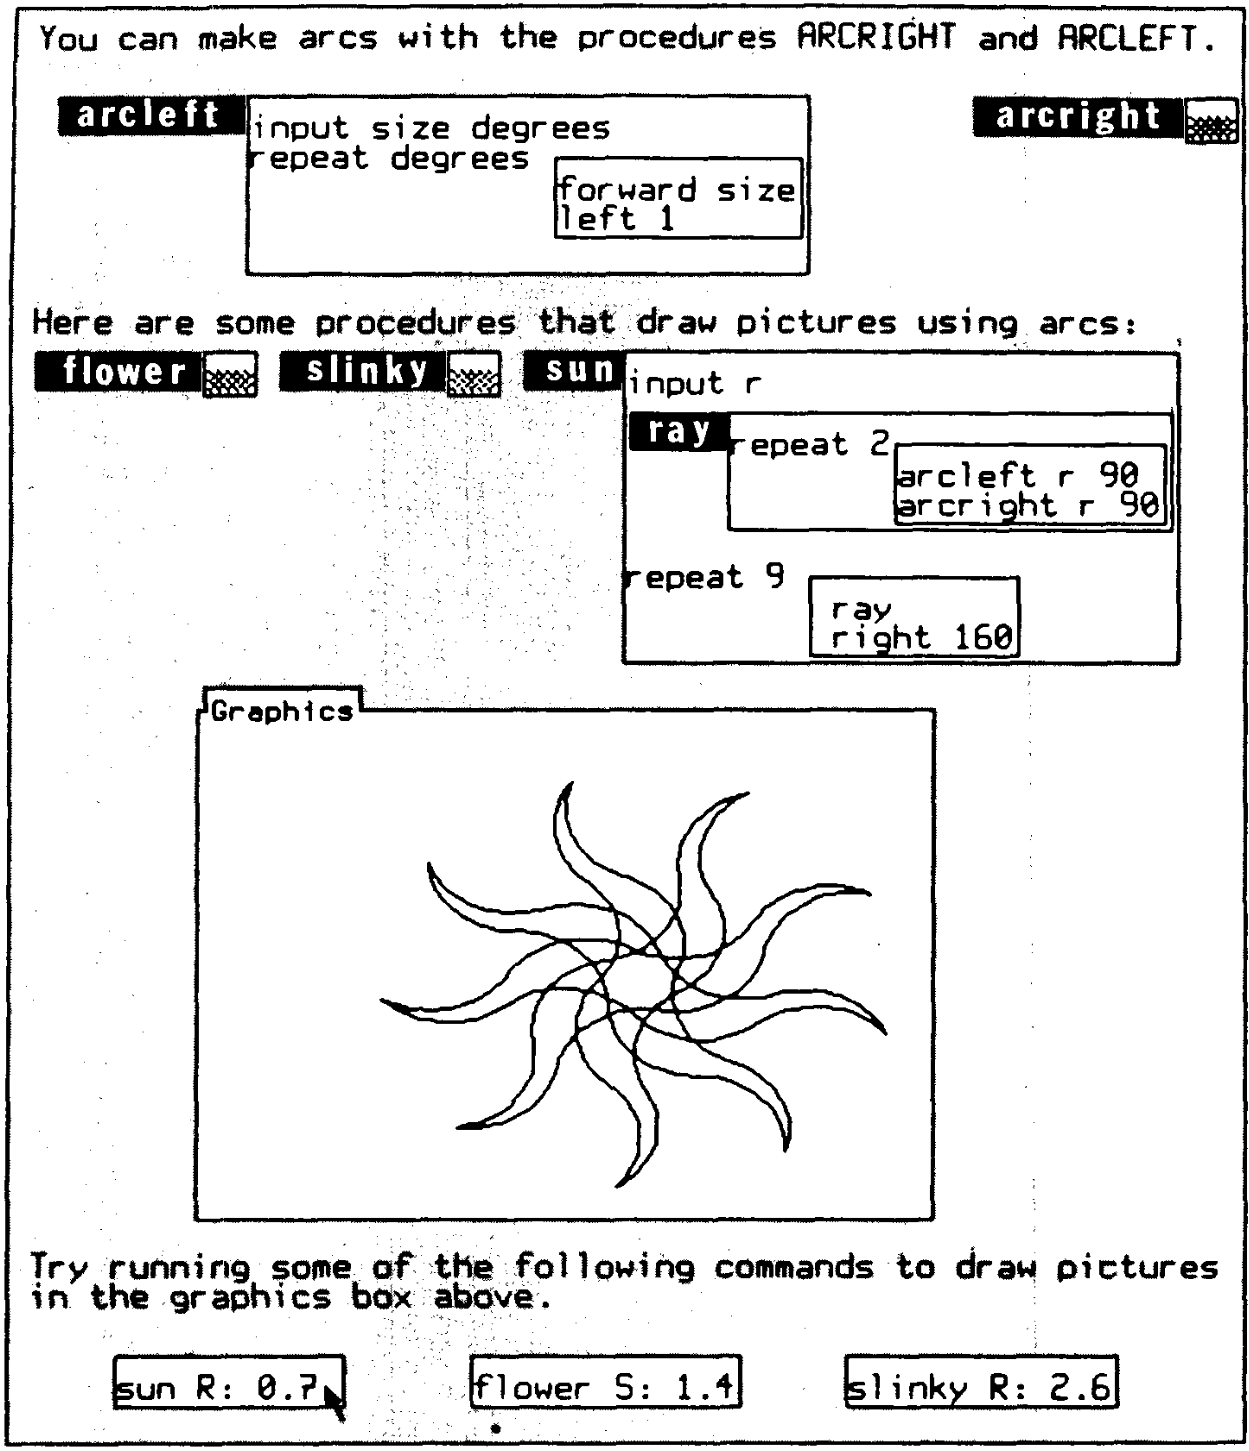
\includegraphics[width=\linewidth]{fig/boxer.png}
  \end{minipage}
  \hfill
  \begin{minipage}{0.57\textwidth}
  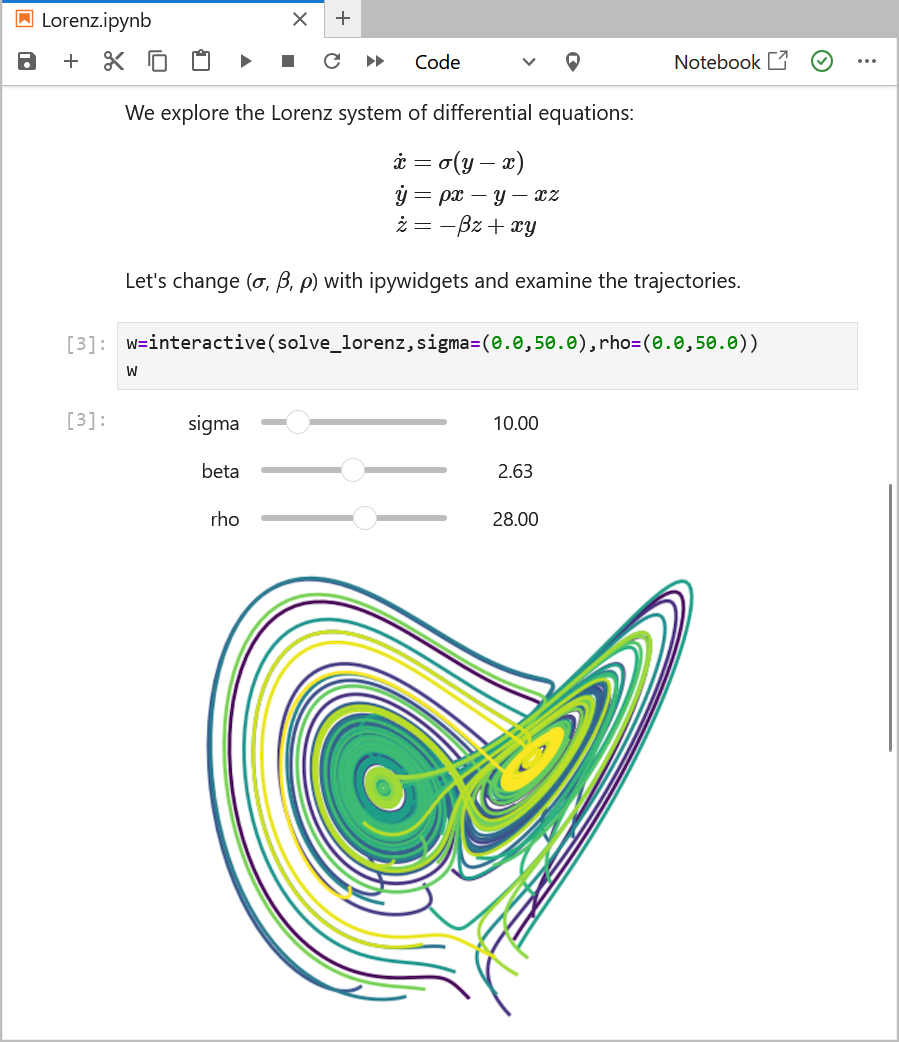
\includegraphics[width=\linewidth]{fig/jupyter.png}
  \end{minipage}
\end{wide}
\vspace{-0.5em}
\caption{%Two examples of document-oriented programming systems.
In Boxer \cite{disessa-1986-boxer}
(left), code and data are represented as nested boxes. All code and state exists in the document.
Executing a box runs the code, which can make changes to the document.
In Jupyter \cite{kluyver-2016-jupyter} (right), documents consist
of sequence of cells. The results of evaluating a code cell are displayed in the document, but the
full state is managed by the hidden underlying kernel.}
\label{fig:systems}
\end{figure}

\section{Introduction}
\label{sec:intro}
Document-oriented programming systems are programming environments that are built around a user
interface modelled after a document editor. The document interface is typically used
for editing the underlying program, for executing the program or its fragments, as well as
for using interactive elements embedded in the document. The origins of the paradigm can be
traced to the 1980s \cite{disessa-1986-boxer} and the paradigm has a rich history, but there has
been a renewed interest in the design of document-oriented programming systems in recent years,
both in practice and in research (Figure~\ref{fig:systems}).

As historical, as well as recent, examples of document-oriented programming systems illustrate,
there are many ways in which the document metaphor can be used as the basis for a programming
system. In particular, there is a great variety in the kind of document structure used,
in how rich user interfaces are embedded within the document, in how programming is integrated
with the document and also in how computations are executed.

We argue that to advance research on document-oriented programming systems, we need to (i)~precisely
characterise what a document-oriented programming system~is, (ii) understand the design
choices available to the designers of document-oriented programming systems, and (iii)
document the design choices made in existing document-oriented programming systems.

\subsection{Definition}
\label{sec:def}
The term \emph{programming system} has been used to talk about ``an integrated and complete set of tools
sufficient for creating, modifying, and executing programs''~\cite{jakubovic-2023-techdims}.
The term shifts the focus from programming languages to a more general notion that also encompasses
the interactive graphical environments in which programming is done.

Document-oriented programming systems are a particular kind of programming systems, built around
the central metaphor of a document. Such systems represent programs as documents that include data,
code, documentation, but sometimes also evaluation state and other artefacts. The programming and
using of programs in a document-oriented programming system is also done through the
document interface.

To make the category of document-oriented programming systems more precise, we use
Technical Dimensions of Programming Systems \cite{jakubovic-2023-techdims}. The framework
identifies a number of axes along which programming systems can be placed and contrasted.
Document-oriented programming systems occupy a particular sub-space of the entire design
space mapped by the technical dimensions framework. The sub-space can be delineated in terms
of three main categories of technical dimensions.

\begin{itemize}
\item \textbf{Notation.} The \emph{primary notation} in a document-oriented programming system
is a document. Many systems are based on structured text documents, but some include
other media such as images or video. Other document structures include spreadsheets,
stacks of cards or text-based Markdown documents. The document often includes
\emph{secondary notations} representing formulas or code, possibly in multiple different
programming languages. The \emph{notational structure} is thus built around multiple
complementing notations.

\item \textbf{Interaction.} In the main \emph{mode of interaction} in document-oriented
programming systems, the user cam modify the document, edit and execute code embedded in the
document and also interact with any interactive elements in the document. The effects of interacting
with the document are mostly immediate, although only a few systems are live. The \emph{feedback
loops} in document-oriented programming systems thus typically aim to minimize the gulf of
evaluation. Within the main mode of interaction, there may be multiple more specific sub-modes,
for example when editing code in a code editor embedded within the document.

\item \textbf{Customization.} In document-oriented programming systems, it is typically possible
to modify the document at any point during the use of the system. In terms of technical
dimensions, the \emph{staging of customization} is such that that the modification of the
document or code embedded in it does not require a special \emph{mode of interaction}. The
customization is also done using the original notations of the system. However, it is rarely
possible to modify the system itself from within the document and this typically requires a
different mode of interaction (such as editing system source code outside of the document
and restarting the system).
\end{itemize}

The aforementioned aspects define \emph{document-oriented programming systems}.
While the design space can be further mapped using existing technical dimensions,
many design choices that are specific to document-oriented programming systems,
are not included in the framework and a deserve further examination.

\subsection{Contributions}
Technical dimensions of programming systems \cite{jakubovic-2023-techdims} map the broad
design space of programming systems. As the authors pointed out, programming systems built
around text-based programming languages form one well-understood cluster in the space.

In this paper, we identify and zoom in on another interesting cluster of programming systems.
Document-oriented programming systems deserve a close examination. The systems in this cluster
share multiple technical characteristics and often aim to make programming more accessible.
They have a rich history, include some of the most widely used programming systems (spreadsheets)
and form an active research area.

\begin{itemize}
\item We characterize the notion of a document-oriented programming system in terms of the
  technical dimensions framework (Section~\ref{sec:def}), going beyond the informal metaphor
  of a programming system built around a structured document.
\item We review a number of diverse past and recent examples of document-oriented programming
  systems (Section~\ref{sec:examples}). These provide valuable reference points for discussion
  about system design.
\item We present a catalogue of twelve central design choices that designers of document-oriented
  programming systems face (Sections~\ref{sec:struct}, \ref{sec:prog}, \ref{sec:gui}, \ref{sec:eval}),
  alongside with interesting examples illustrating the different choices.
\end{itemize}

To develop the catalogue, we draw from our own experience developing multiple document-oriented programming systems
\cite{jakubovic-2022-bootstraplab,petricek-2025-denicek,edwards-2005-subtext,edwards-2025-baseline,edwards-2018-directprog},
extensive literature review and also discussions at multiple workshops dedicated to past and
future programming systems (Boxer Salon 2022, Substrates 2025).

\subsection{Using this Paper}

Tha aims of this paper are to highlight an interesting programming systems paradigm, develop a better
understanding of the design choices within the paradigm and facilitate further research on
document-oriented programming systems. The different aims are best served by different ways of
using the paper.

\begin{itemize}
\item Readers who want to get an overview of document-oriented programming systems can
  focus on the introduction (\S\ref{sec:intro}) and examples (\S\ref{sec:examples}). They can then
  read the summary paragraphs for each of the design choices and learn about interesting designs
  by examining the examples (``Example'' sections) throughout the paper.

\item Researchers who are interested in comparing document-oriented programming systems
  can read the summary paragraphs for each of the design choices and then proceed to the
  details of the design choices that are relevant for their systems.

\item Designers of novel document-oriented programming systems may find it useful to skim through
  the entire catalogue to explore interesting, but under-researched alternatives to some of the
  widely used and established design choices.
\end{itemize}

Although the paper can be read cover to cover, it is better approached with a specific
document-oriented programming system or a design question in mind.

\section{Examples}
\label{sec:examples}
There are many programming systems that match our definition of a \emph{document-oriented
programming system}. In this section, we provide a brief overview of some of them, focusing on
systems that appear frequently as examples in our catalogue.

\begin{figure}[b]
\centering
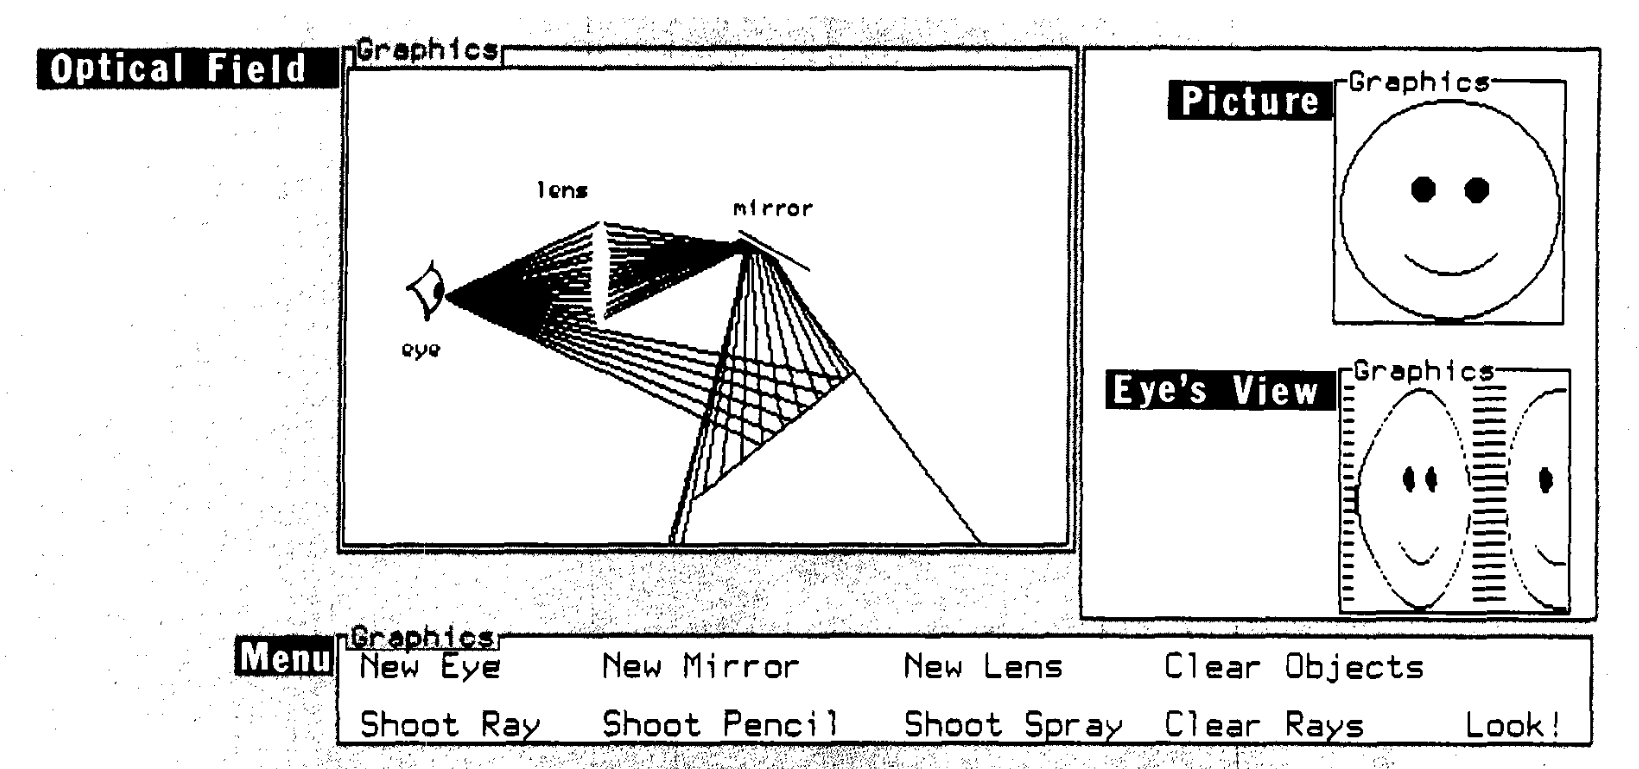
\includegraphics[width=0.95\linewidth]{fig/optics.png}
\caption{A page from a Boxer textbook on optics. Readers can construct new experiments, but
  also explore the implementation. (Image source~\cite{disessa-1986-boxer})}
\label{fig:book}
\vspace{1em}
\end{figure}

\subsection{Historical Origins: Boxer}
The Boxer system \cite{disessa-1986-boxer,disessa-1985-design} was developed in the early 1980s
as an educational interactive computational environment. One of the envisioned use cases of
the system was production of interactive textbooks. The readers of such textbook would be able
to explore interactive explanations in the textbook, modify parameters, but also see the
logic implementing the explanations and potentially customize it (Figure~\ref{fig:book}).

In Boxer, the document consists of nested boxes. There are two main kinds of boxes.
{\sc Data} boxes contain text, graphics and other boxes. {\sc Doit} boxes contain program
text and other {\sc Doit} and {\sc Data} boxes \cite[p.2]{klotz-1989-boxer}. Boxes are used
to represent structured data (such as a collection of records) as well as nesting structure
in code (body of a loop). The system also includes {\sc Graphics} boxes that can display
visual output and respond to user interactions.

The Boxer environment lets the user manipulate the document. They can create new boxes, modify
text and code in existing boxes and delete boxes. Boxer uses \emph{spatial metaphor},
leveraging the commonsense knowledge of space to make computing more comprehensible
\cite[p.2]{disessa-1986-boxer}. Another important principle of Boxer is \emph{naive realism},
which means that what the users see on their screen is ``their computational world in its
entirety'' \cite[p.3]{disessa-1986-boxer}. Boxes can be shrunk to hide their contents and
even put in closets to hide them \cite{disessa-2021-structures}, but they are always present
in the document and can always be located and accessed.

Computation in Boxer is represented as code in {\sc Doit} boxes. The code can be executed by
clicking on the box. Conceptually, evaluation of code is based on \emph{copying semantics}.
When the running code references another box, the evaluation behaves as if the referenced box
was copied in the place where it is referenced from. (The consequence of this model is that
the system uses dynamic variable scoping.) Computation can modify state of the document. If
it also produces a result, the result is placed in a new {\sc Data} box in the document.

Boxer also provides a range of functions for manipulating boxes in the document.
For example, the \texttt{BUILD} command can be used to construct a new box from a box
that serves as a template with placeholders, in a manner similar to meta-programming in Lisp.
However, the underlying Boxer runtime that provides the basic user interface and evaluation
logic remains hidden from the user and cannot be modified directly from within Boxer.

\begin{figure}[t]
\begin{wide}
\centering
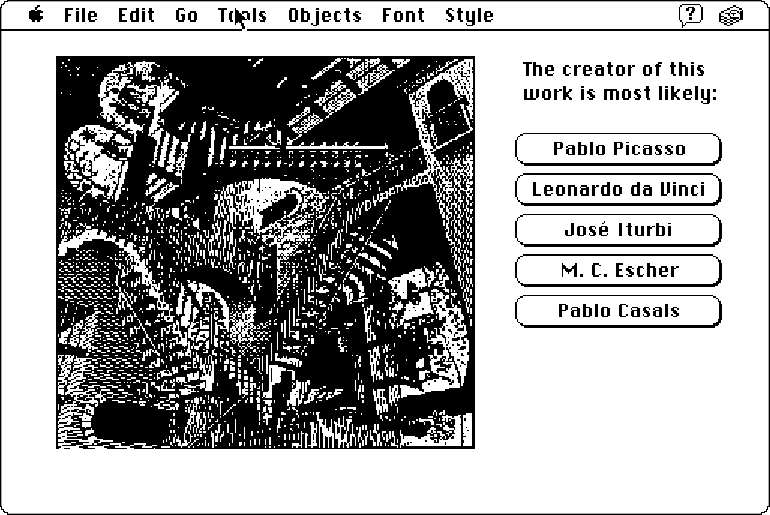
\includegraphics[width=0.48\linewidth]{fig/hyper1.png}
\hfill
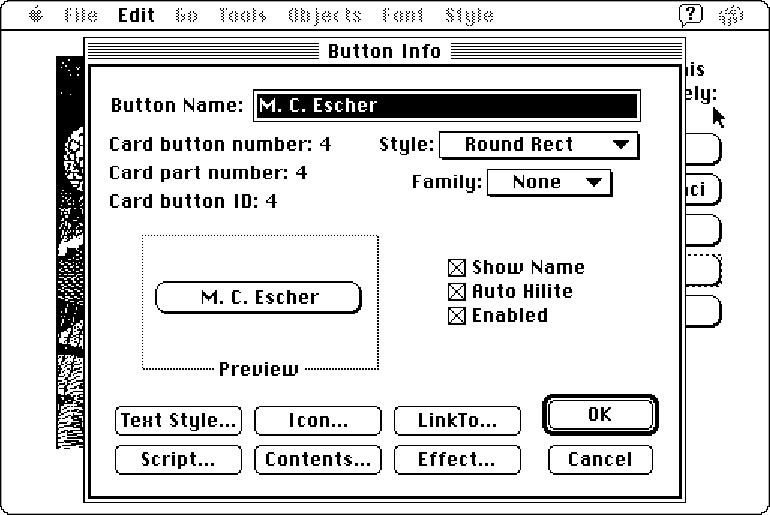
\includegraphics[width=0.48\linewidth]{fig/hyper2.png}
\end{wide}
\caption{HyperCard. (Screenshot from Archive.org \cite{countant-1994-arthistory})}
\label{fig:hyper}
\end{figure}

\subsection{Successful: HyperCard, Spreadsheets and Jupyter}
\paragraph{HyperCard}
\paragraph{Spreadsheets}
\paragraph{Jupyter}

\subsection{Current Research: Subtext and BootstrapLab}
subtext \cite{edwards-2005-subtext}
see the direct programming video - https://vimeo.com/274771188

list of edits
tree of records and lists
live evaluation of formulas like spreadsheets
code (formula / ast) is also a record with fields for individual operations
functional model
native GUI with no custom projections
evaluation is live
final state is an annotation added to the doc

\subsection{BootstrapLab}
xx



\newpage

\section{Design Choices: Structure}
\label{sec:struct}
The first set of design choices relates to the structure of the document.
They determine what kind of document the user sees and works with, as well as how
the document is represented internally by the system.

\subsection{Document Shape}
\label{sec:struct-shape}
The document shape is the visible structure that the user manipulates and interacts
with. This is the primary visible notation of the system. In many document-oriented
programming systems, the shape is a tree consisting of different kinds of nodes.

\begin{itemize}
\item \emph{Tree-Shaped Documents.} The tree can be displayed directly to user using
  some form of tree view widget that lets users directly manipulate the tree
  (Subtext \cite{edwards-2005-subtext}, BootstrapLab \cite{jakubovic-2022-bootstraplab}).
  The tree can be modelled after (or built directly on top of) structured mixed-media
  documents such as HTML (Webstrates \cite{klokmose-2015-webstrates}, Webnicek \cite{petricek-2025-denicek}),
  in which case the user can often view and edit the document directly (WYSIWYG) or
  through a source view (tree view widget).

\item \emph{Sequence of Cells.} Computational notebooks for data science
  (Jupyter \cite{kluyver-2016-jupyter}, Wrattler \cite{petricek-2018-wrattler}, Datnicek \cite{petricek-2025-denicek})
  and programming systems built for journalist (Idyll \cite{conlen-2018-idyll},
  Planet Hazel \cite{bandukwala-2024-planet}, The Gamma \cite{petricek-2015-journalism})
  use a flat structure where the document is a sequence of cells of different kinds,
  including textual cells, code cells, interactive cells or outputs of a computation.

\item \emph{Two-Dimensional Grid.} In spreadsheet systems \cite{abraham-2009-spreadsheets},
  the document shape is a regular two-dimensional grid. Cells in the grid can contain data and
  formulas. In some systems, other structures are overlaid over the grid (such as named ranges)
  and there may be a secondary notation (macro language).

\item \emph{Other Choices.} Other choices are less common.
  HyperCard \cite{atkinson-1987-hypercard} documents are stacks of cards, which can contain
  freely positioned graphical, textual and interactive elements. An unstructured representation
  is used in Potluck \cite{litt-2022-potluck}, where the document is a plain-text Markdown
  document (although rendered as rich text).
\end{itemize}

\vspace{-0.5em}
\paragraph{Example: Ampleforth.}
In Ampleforth~\cite{bracha-2022-ampleforth}, the document shape is not fixed beforehand.
The Ampleforth system is embedded in the live programming environment of the object-oriented
programming  language Newspeak \cite{bracha-2025-newspeak}, which runs in the web browser.

Internally, Ampleforth documents are Newspeak objects, but they are displayed as rich text
documents containing media (using standard capabilities of the web browser) and also
interactive Ampleforth elements (which send messages to the underlying Newspeak objects).
An Ampleforth document can thus have many different specific shapes. As illustrated by the
DocuApps project \cite{bracha-2024-docuapps}, this includes structured documents, presentation
slides and spreadsheets.

The BootstrapLab~\cite{jakubovic-2022-bootstraplab} system has a similar capability.
Its underlying representation is a graph (primarily a tree, but with arbitrary links),
but what is displayed to the user can be reprogrammed within the system itself. The example
implemented in the prototype is a tree view, but other renderings are possible.

\subsection{Document Representation}
\label{sec:struct-repr}
Whereas \emph{Document Shape} is concerned with the user-facing side of a document-oriented
programming system, \emph{Document Representation} focuses on the internal data structures that
the system maintains. In the technical dimensions framework \cite{jakubovic-2023-techdims},
the two aspects are referred to as \emph{surface notation} and \emph{internal notation}.

\begin{itemize}
\item \emph{Document Itself.} In many systems, their internal
  notation closely resembles to the surface notation and what they display to the user is a
  direct rendering of their document representation (Boxer~\cite{disessa-1986-boxer},
  HyperCard~\cite{atkinson-1987-hypercard}, Jupyter~\cite{kluyver-2016-jupyter}).

\item \emph{Underlying Model.} Document-oriented programming systems can be embedded in
  another programming system with a more basic underlying representation. This can be a
  soup of objects (Ampleforth~\cite{bracha-2022-ampleforth}) or a graph
  structure (BootstrapLab~\cite{jakubovic-2022-bootstraplab}).

\item \emph{Edit History.} In a number of systems, the ground truth is not the document itself,
  but a sequence of edit operations through which the document has been created
  (Subtext~\cite{edwards-2018-directprog,edwards-2021-typed}, Denicek~\cite{petricek-2025-denicek}).
  The document is computed by reapplying the operations, but the history can be used
  to implement programming by demonstration.
\end{itemize}

\paragraph{Example: Webstrates.}
In Webstrates~\cite{klokmose-2015-webstrates}, there is no gap between the \emph{internal notation}
and the \emph{surface notation}. The Webstrates system is built on top of the web platform and
it uses the web browser's Document Object Model (DOM) as the canonical document representation.
Webstrates make the document collaboratively editable by synchronizing it between devices.
However, editing is done directly to the document through the browser developer tools or through
Codestrates~\cite{radle-2017-codestrates}, which is a development platform built on top of
Webstrates.

\subsection{Modularity}
The choice of modularity mechanism determines how can aspects of programs be reused. The design
choice corresponds directly to the technical dimension \emph{factoring of complextiy}.
In programming languages, this is often the key concern and possible solutions range from
classes and inheritance to domain-specific languages and type classes. In document-oriented
programming systems, most programs are more direct and only implement more basic modularity
mechanisms (possibly posing an interesting open question for the future of the paradigm).

\begin{itemize}
\item \emph{Transclusions.} Transclusions \cite{nelson-1981-litmachines} is a hypertext concept,
  where a resource, or a part of a document, is included in multiple different places at once.
  In document-oriented programming systems, they allow modularity without introducing additional
  concepts (such as a function call) to the end-users. They can be used to reuse a component
  existing inside the document (Boxer~\cite{disessa-1986-boxer}), as well as content that may
  exist elsewhere in the underlying model (Ampleforth \cite{bracha-2022-ampleforth}).

\item \emph{Internal References.} A more basic mechanism for modularity and code reuse is a
  reference to an entity defined elsewhere in the document. (See \S\ref{sec:eval-ident} for
  different referencing mechanisms.) Unlike with transclusions, the entity is not displayed in the
  document location where it is referenced (the user typically sees the entity name). The
  reference can refer to functions (BootstrapLab~\cite{jakubovic-2022-bootstraplab}),
  interactive components (Livelits~\cite{omar-2021-livelits}), or more generally ancestral
  nodes (Subtext~\cite{edwards-2005-subtext}).

\item \emph{External References.} In many document-oriented programming systems, the ability to
  define new abstractions within the document is limited and so modular components or code
  are defined outside of the document. Those can be external libraries (Jupyter~\cite{kluyver-2016-jupyter})
  or interactive components (\cite{conlen-2018-idyll}).

\item \emph{Edit History Reference.} In systems where the underlying representation of a document
  is a history of edits (see \S\ref{sec:struct-repr}), it is also possible to spcify behavior
  by referring to a part of the history (replaying the edits then performs the behavior again).
  The mechanism can be used to implement programming by demonstration \cite{cypher-1993-pbd}
  (Subtext \cite{edwards-2005-subtext}, Denicek \cite{petricek-2025-denicek}).
\end{itemize}

\begin{figure}[t]
\hspace{5em}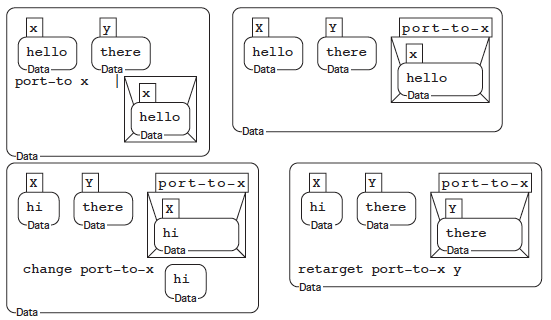
\includegraphics[width=0.8\linewidth]{fig/ports.png}
\caption{Portals (a transclusion mechanism) in Boxer. A port is created using the
\texttt{port-to} command (left top) and is itself a box that can be named (left right). Changing
the value of the portal box changes the original source (bottom left) and portals can be
redirected~(bottom right). Image source \cite{disessa-2021-structures}.}
\label{fig:ports}
\end{figure}

\paragraph{Example: Boxer.}
In Boxer, parts of a document can be reused through ports (Figure~\ref{fig:ports}). They are
views of another box and, despite looking differently, behave identically to their target.
The Boxer Structures report \cite{disessa-2021-structures} lists a number of typical uses of ports.

Ports can be used as a user interface mechanism to provide easy access to another box
hidden somewhere in the document, or to create an easy to follow hyperlink. They can be used
to share data between parts of a document. Ports are also useful as object references, for example
to create a list of objects (existing elsewhere in a document) to be processed. Although
Boxer supports named references to variables and procedures, ports can also be used for this
purpose to avoid name mix-ups.

\begin{figure}[t]
\begin{wide}
  \centering
  \begin{minipage}[t]{0.38\textwidth}\vspace{0pt}
  {\footnotesize \textbf{(a)} Sequence of instructions}

  \vspace{1em}
  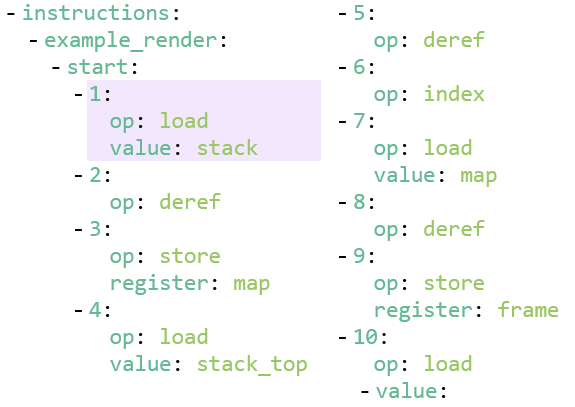
\includegraphics[scale=0.38]{fig/blab-instr.png}
  \end{minipage}
  \hfill
  \begin{minipage}[t]{0.38\textwidth}\vspace{0pt}
  {\footnotesize \textbf{(b)} Textual MASP notation}

  \vspace{1em}
  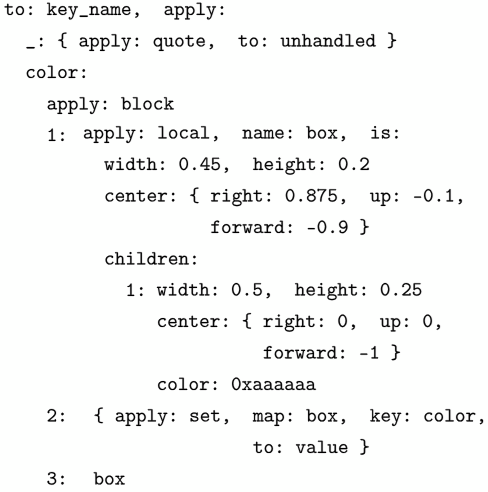
\includegraphics[scale=0.4]{fig/blab-masp.png}
  \end{minipage}
  \hfill
  \begin{minipage}[t]{0.38\textwidth}\vspace{0pt}
  {\footnotesize \textbf{(c)} Box-based MASP notation}

  \vspace{1em}
  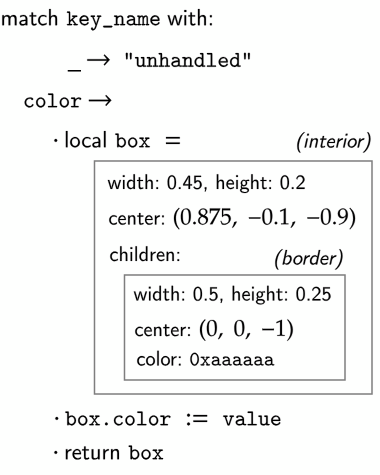
\includegraphics[scale=0.4]{fig/blab-vis.png}
  \end{minipage}
\end{wide}
\caption{Two different programming models in BootstrapLab~\cite{jakubovic-2022-bootstraplab}.
\textbf{(a)} Imperative instructions to mutate document that read the top of a stack and store the
result in a register (a special document node). \textbf{(b)} A functional document transformation
that replaces \texttt{color} field with a filled rectangle that has the given color. \textbf{(c)}
Visual rendering of the same MASP code. (Image source \cite{jakubovic-2024-self})}
\label{fig:blab}
\end{figure}

\section{Design Choices: Programming}
\label{sec:prog}
An essential characteristic of document-oriented programming systems is that they allow some
kind of programming. However, our definition admits both end-user document systes with
limited programming capabilitie and systems that can be fully reprogrammed from within themselves.
Systems also differ in their programming model, as well as where and how they store program code.

\subsection{Programming Model}
\label{sec:prog-model}
The basic programming model of a document-oriented programming system can be built around the
standard programming language paradigms.

\begin{itemize}
\item \emph{Imperative.} In the imperative programming model, code embedded in the document
  consists of operations that mutate some state (see \S\ref{sec:eval-state}). In some
  systems, commands can modify the document itself (HyperCard~\cite{atkinson-1987-hypercard},
  Ampleforth \cite{bracha-2022-ampleforth}, Boxer~\cite{disessa-2021-structures},
  Webstrates~\cite{klokmose-2015-webstrates}), while in others, commands can only modify state
  that exists behind the scene but not the document structure (Jupyter \cite{kluyver-2016-jupyter}).

\item \emph{Declarative.} In the declarative model, code in the document describes a computation
  that should be performed in order to obtain some result (Subtext~\cite{edwards-2005-subtext},
  Spreadsheets~\cite{abraham-2009-spreadsheets}). The result may be displayed alongside
  the document, or placed in the document (see \S\ref{sec:eval-state}), but the code
  does not explicitly modify the document.

\item \emph{Reactive.} When the declarative programming model makes it possible to write code that
  explicitly responds to user interactions with the system, it can be referred to as
  reactive (Renkon-pad~\cite{ohshima-2025-renkonpad}, Lopecode~\cite{larkworthy-2025-lopecodetour}).
  Note that spreadsheets support live updates, but only in response to change of the source (data).

\item \emph{Transformation.} Another variation on the declarative programming model exists in
  systems where computations operate on document fragments and their result is also a document
  fragment. The evaluation may transform the document (Webnicek~\cite{petricek-2025-denicek}),
  but the model has origins in systems that generate new documents as the result
  (XSLT~\cite{clark-1999-xslt}, Document calculus \cite{crichton-2024-document})
\end{itemize}

\paragraph{Example: BootstrapLab.}
BootstrapLab \cite{jakubovic-2022-bootstraplab} shows that a document-oriented programming
system may support multiple different programming models. The primitive programming model in
BootstrapLab is imperative. Code is represented as a sequence of low-level instructions that
modify a set of registers (Figure~\ref{fig:blab} (a)). The instruction pointer register
determines the next instruction to be executed. The programming model includes operations such
as key lookup, copying, and conditional jump.

A high-level programming model envisioned in BootstrapLab is the MASP language, modelled after
LISP (Figure~\ref{fig:blab} (b)). The document structure (nested maps) represents the abstract
syntax tree of functional-first programs. The code can be rendered as textual tree, but also
visually (Figure~\ref{fig:blab} (c)). The MASP interpreter stores all immediate information,
as well as the final result, directly in the document (see~\S\ref{sec:eval-state}).
Although this was not done in the BootstrapLab prototype, a MASP interpreter or compiler
could be built in the low-level programming model.

\subsection{Metaprogramming Capabilities}
\label{sec:prog-meta}

Document-oriented programming systems differ by the degree to which they can be modified
from within themselves. This is known as \emph{self-sustainability} in the technical dimensions
framework \cite{jakubovic-2023-techdims}. As most document-oriented programming systems are not
self-sustainable (i.e., not implemented and modifiable from within themselves), we
refer to the design choice as \emph{Metaprogramming Capabilities}.

\begin{itemize}
\item \emph{No Metaprogramming.} In many document-oriented programming systems, computation can
  only produce results that are displayed in the document (Spreadsheets~\cite{abraham-2009-spreadsheets},
  Idyll \cite{conlen-2018-idyll}, Potluck \cite{litt-2022-potluck}).
\item \emph{Limited Metaprogramming.} In most notebook systems, code written by the user cannot
  arbitrarily modify the structure of the notebook, but there may be a special operation
  for, for example, adding a new cell (Jupyter \cite{kluyver-2016-jupyter},
  Observable \cite{observable-2025-hq}).
\item \emph{Document Metaprogramming.} In a number of document-oriented programming systems, code
  running in the system has the capabilities to freely modify the structure of the document,
  but it cannot modify the system itself (HyperCard \cite{atkinson-1987-hypercard},
  Webstrates \cite{petricek-2018-wrattler}, Wrattler \cite{petricek-2018-wrattler}, Boxer \cite{disessa-1986-boxer}).

\item \emph{Full Metaprogramming.} Only document-oriented programming systems where much of the
  system itself is implemented within itself can be modified from within code in the document.
  (Ampleforth \cite{bracha-2022-ampleforth}, BootrstrapLab \cite{jakubovic-2022-bootstraplab},
  Lopecode \cite{larkworthy-2025-lopecodetour}). The degree depends on what the minimal
  unmodifiable runtime of the system is.
\end{itemize}

\paragraph{Example: Lopecode.}
Metaprogramming capabilities of most notebook systems are very limited, but Lopecode~\cite{larkworthy-2025-lopecodetour}
shows that this is not inevitable. The system is built on top of the reactive kernel
from Observable~\cite{observable-2025-hq}, which maintains a dataflow graph of the computation.
Everything else, including the document model based on cells and the editor is implemented
(and can be modified from) Lopecode notebooks.

\subsection{Code Representation}
How is code represented in a document-oriented programming system and where can it be found?
We consider these two aspects together as a signle design choice.

\begin{itemize}
\item \emph{Naive Realism} vs. \emph{Hidden Representation.} In the naive realism model,
  everything that exists in the system is available in the document (Boxer \cite{disessa-1986-boxer},
  Jupyter \cite{kluyver-2016-jupyter}, Subtext \cite{edwards-2005-subtext}).%\footnote{The
  %term \emph{naive realism} has been coined by diSessa in the context of Boxer.}.
  In contrast, systems where code exists outside of the document use the
  hidden representation model (HyperCard \cite{atkinson-1987-hypercard},
  Ampleforth \cite{bracha-2022-ampleforth}).

\item \emph{Structured Representation} vs. \emph{Textual Representation.}
  Most document-oriented programming systems use a structured representation of a document,
  such as a tree (see \S\ref{sec:struct-shape}). In such systems, code can be represented as an
  AST using the same structure and edited using a strucute editor (Boxer~\cite{disessa-1986-boxer},
  Subtext~\cite{edwards-2005-subtext}, Denicek~\cite{petricek-2025-denicek}, Hazel~\cite{omar-2021-livelits}).
  The alternative is to use a textual representation of code alongside with an (embedded)
  text editor (Jupyter~\cite{kluyver-2016-jupyter}, Potluck \cite{litt-2022-potluck},
  Ampleforth \cite{bracha-2022-ampleforth}).
\end{itemize}

\subsection{Document Structure Checking}
In programming languages, static typing is the most common mechanism for early \emph{error
detection} (see technical dimensions \cite{jakubovic-2023-techdims}). In document-oriented
programming systems with \emph{Document} or \emph{Full Metaprogramming}
(see \S\ref{sec:prog-meta}), it is possible to use a mechanism akin to type checking to
ensure that operations transforming the document result in a well-formed document structure.

Documents manipulated by systems that use the \emph{Tree-Shaped Document} model
(see \S\ref{sec:struct-shape}) may be irregular containing, for example, different structure
of data in different document sections. As such, it is also an interesting problem to define
what is considered a well-formed document structure.


\begin{itemize}
\item \emph{Minimal Structure.} Systems where document structure is very regular
  (Spreadsheets~\cite{abraham-2009-spreadsheets}) do not typically need sophisticated structure
  checking to ensure the document is well-formed (but even they have possible constraints, such
  as cycles). In computational notebooks (Jupyter \cite{kluyver-2016-jupyter}), checking may
  be useful for the embedded code, but not to ensure the well-formedness of the notebook structure.

\item \emph{Implicit Structure.} Document systems that let users programmatically manipulate
  documents with more complex shapes may allow arbitrary modifications of the structure
  (Webnicek~\cite{petricek-2025-denicek}, BootrstrapLab~\cite{jakubovic-2022-bootstraplab}).
  Changing the structure in a way that is incompatible with other code in the document then
  results in a runtime error, reported when the other code is executed.

\item \emph{Explicit Structure.} In some systems, the document structure can be explicit
  using a mechanism such as a type system or using prototypes. This is an under-explored area of
  research in programming systems (Subtext'21 \cite{edwards-2021-typed}), but examples
  exist in document manipulation (XDuce \cite{hosoya-2003-xduce}, Ur/Web \cite{chlipala-2015-urweb}).
\end{itemize}

\paragraph{Example: Subtext 10 and Baseline.}
An example of a system with explicitly checked document structure is Subtext~10~\cite{edwards-2021-subtext10}
(which served as the basis for a more recent prototype implementation Baseline~\cite{edwards-2025-baseline}).
Subtext 10 uses a form of static type checking that is based on concrete values. The type of a
collection is determined by a special element (with index \texttt{*}) that serves as a default
value (or a prototype \cite{borning-1986-prototypes}).

The default value is used when adding a new
item to the collection to ensure that all items have the same structure. Similarly, a structural
document edit (e.g., adding, renaming or removing a record field) can only be applied to the
default value and results in the change being applied to all items of the collection.
In Subtext 10, default values were also proposed for function arguments.

\section{Design Choices: Graphical Interface}
\label{sec:gui}

Whereas some of the design choices related to structure (\S\ref{sec:struct}) and
programming~(\S\ref{sec:prog}) coincided with the more general technical dimensions
\cite{jakubovic-2023-techdims}, the design choices concerning user interface are
new in this paper. We consider two complementary mechanisms, for display and for editing.

\subsection{Display Mechanism}
A defining characteristic of document-oriented programming systems (\S\ref{sec:def})
is that the user sees and interacts with a document. There are multiple display mechanisms
through which the document can appear on screen.

\begin{itemize}
\item \emph{Naive Realism.} Systems where the document representation is the document
  itself, or edit history from which the document is obtained (see \S\ref{sec:struct-repr}),
  the system may have a standard mechanism for displaying the document
  (Boxer~\cite{disessa-1986-boxer}, Webstrates~\cite{klokmose-2015-webstrates}, Webnicek~\cite{petricek-2025-denicek}).
  Custom graphical elements can be constructed using components of the standard mechanism
  such as graphics boxes \cite{disessa-2021-structures} or HTML.

\item \emph{Renderer with Widgets.} In systems where the document representation is less
  expressive, custom graphical elements can be implemented as widgets that are defined outside
  of the document itself. They can then be created programatically from within the document
  or used automatically to display (end edit) specific types of values. (Livelits~\cite{omar-2021-livelits},
  Jupyter Widgets~\cite{jupyter-2025-widgets}).

\item \emph{API Calls.} Document-oriented programming systems where code exists outside of the
  document can modify the displayed document through some API provided by the system, for example
  to construct document elements and draw (HyperCard~\cite{atkinson-1987-hypercard})
  or generate document fragments (Ampleforth \cite{bracha-2022-ampleforth}).
\end{itemize}

\begin{figure}[t]
\begin{wide}
  \centering
  \begin{minipage}[t]{0.29\textwidth}
  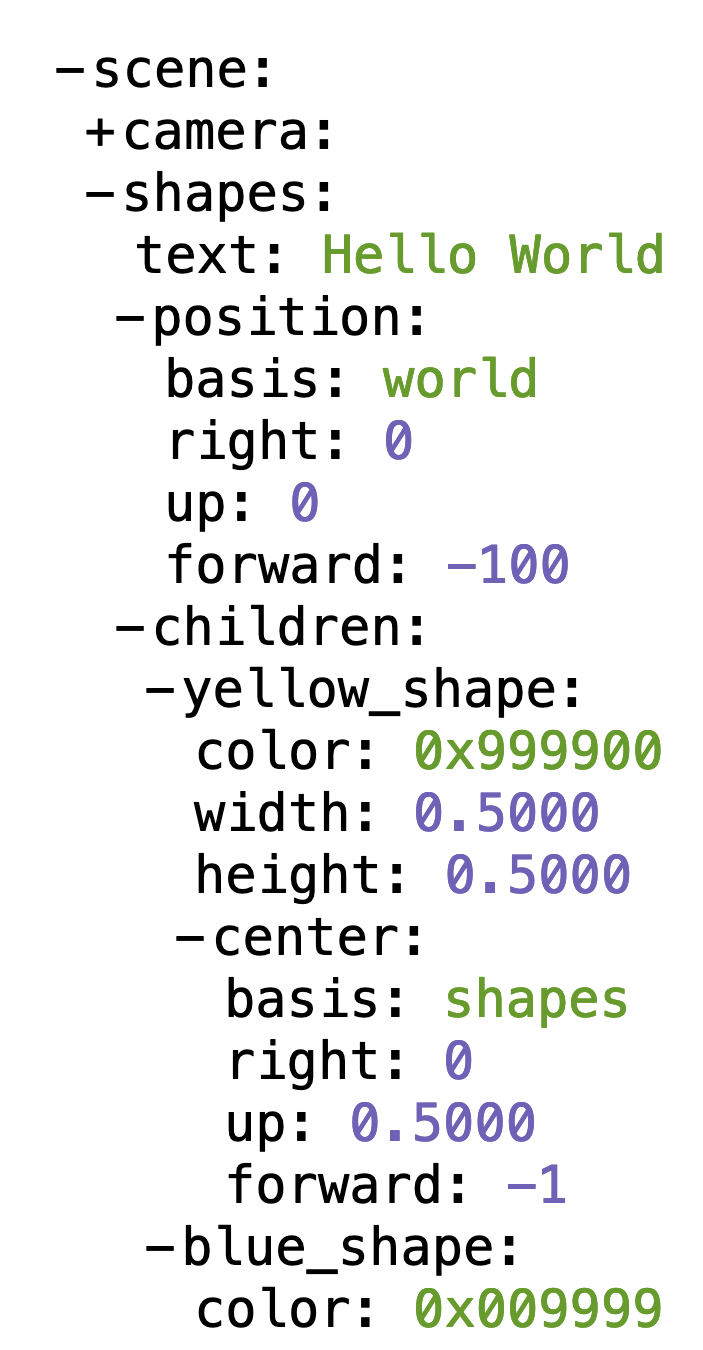
\includegraphics[scale=0.18]{fig/mapped2.png}
  \end{minipage}
  \hfill
  \begin{minipage}[t]{0.29\textwidth}
  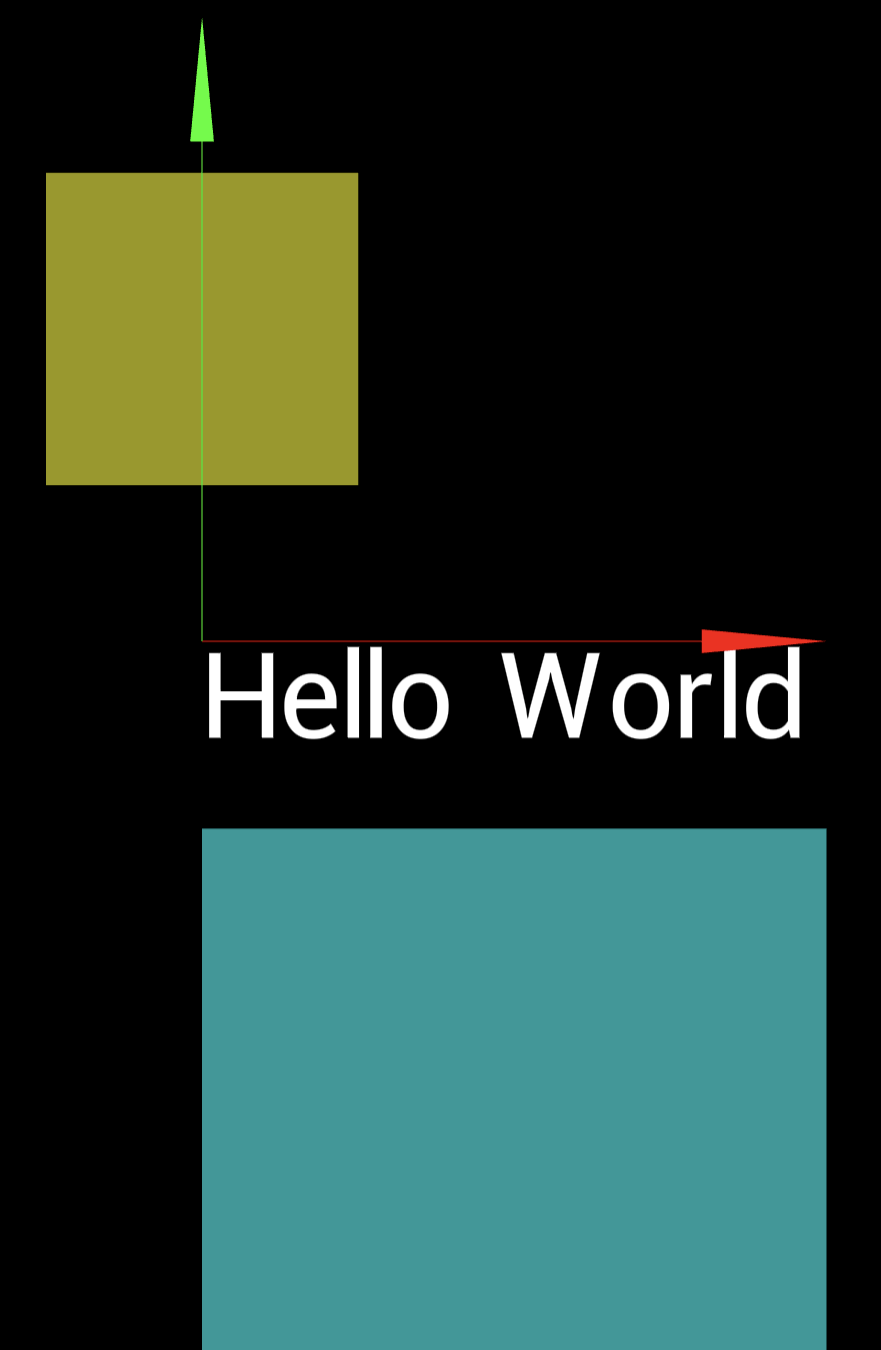
\includegraphics[scale=0.18]{fig/mapped1.png}
  \end{minipage}
  \hfill
  \begin{minipage}[t]{0.27\textwidth}
  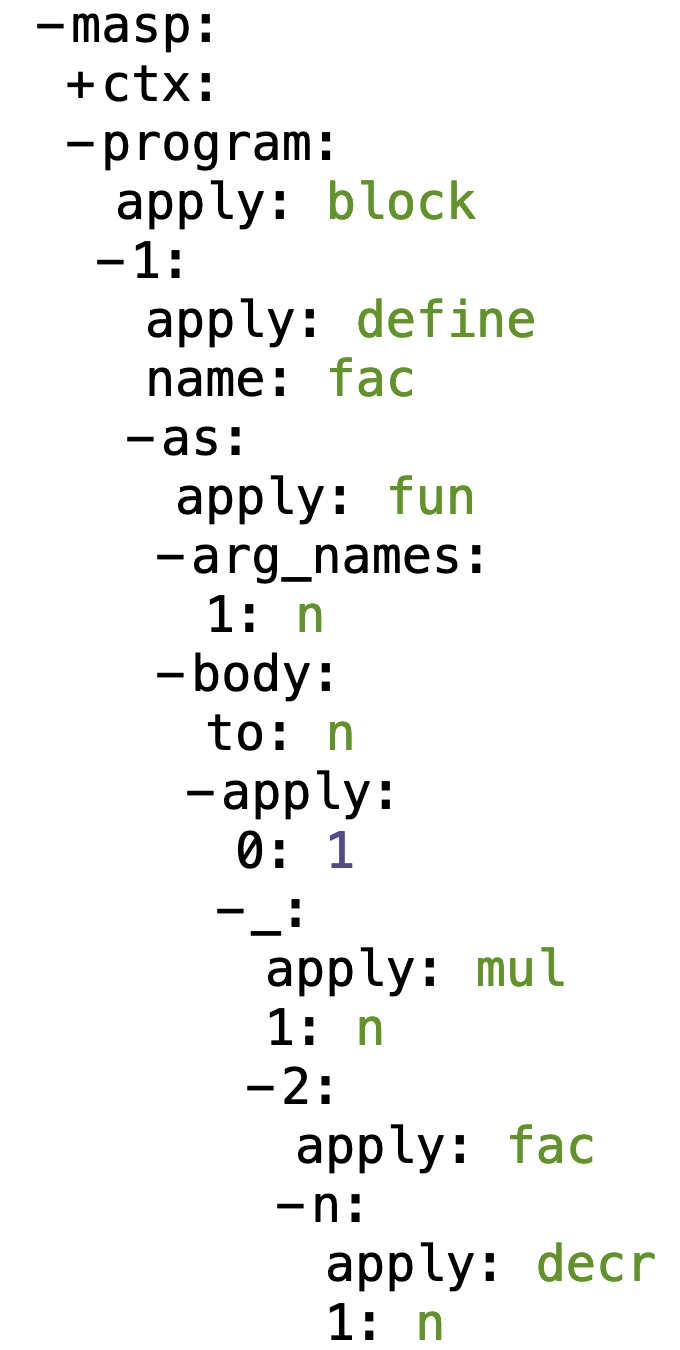
\includegraphics[scale=0.18]{fig/mapped4.png}
  \end{minipage}
  \hfill
  \begin{minipage}[t]{0.27\textwidth}
  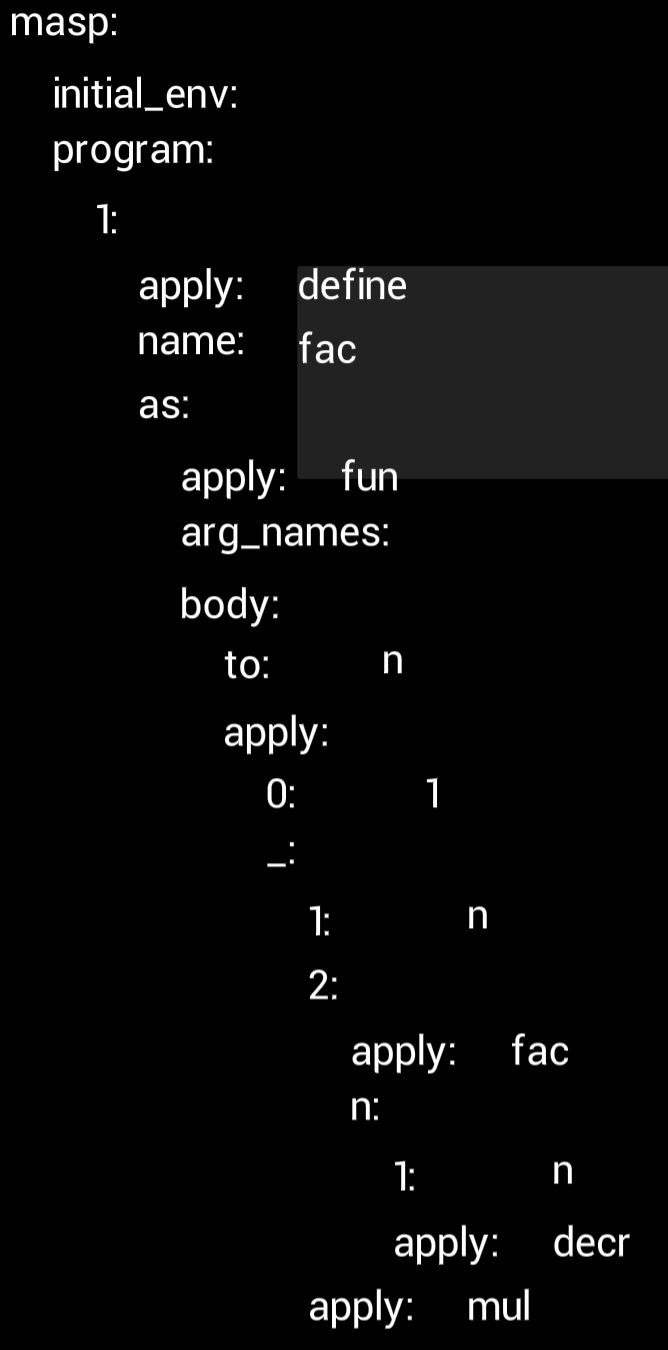
\includegraphics[scale=0.18]{fig/mapped3.png}
  \end{minipage}
\end{wide}
\caption{Memory-mapped display mechanism in BootstrapLab.
  A sample scene consisting of text, rectangles and arrows (a) with rendering (b).
  A tree representing a MASP function, rendered outside of BootstrapLab (c)
  and using the memory-mapped display mechanism (d).
  Image source \cite{jakubovic-2024-self}.}
\label{fig:mapped}
\end{figure}

\paragraph{Example: BootstrapLab.}
An under-explored approach for document rendering has been used in BootstrapLab~\cite{jakubovic-2022-bootstraplab}.
The document in the system is a tree structure consisting of nodes that map keys to other nodes
or primitive values. The document is not displayed directly to the user. Instead, it contains
a special sub-tree (\texttt{scene}) that defines a visual structure to display (as a scene
consisting of vector shapes).

The system can display arbitrary part of the document by filling the \texttt{scene}
sub-tree with shapes rendering the specified sub-tree (Figure~\ref{fig:mapped}).
The mechanism, inspired by memory-mapped screen on microcomputers, makes it possible to keep all
code and data in a tree-shaped document, but fully control what is displayed on the screen.

\subsection{Editing Mechanism}
The editing mechanism used in a document-oriented programming system is usually tightly linked
with the display mechanism. However, it is worth separating the two design aspects as a system
can, for example, display a document visually, but use a plain text editor.

\begin{itemize}
\item \emph{Structure Editing.} Common approach is to let the user directly
  edit the structure of the document through a structure editor that works directly with the
  underlying structure such as tree nodes (Denicek~\cite{petricek-2025-denicek},
  Webstrates~\cite{klokmose-2015-webstrates}, Boxer~\cite{disessa-1986-boxer}).
\item \emph{Projectional Editing.} If the display mechanism lets users construct widgets for
  some parts of the document, the widgets may behave as projectional editors~\cite{voelter-2014-projectional}
  and propagate interactively made edits back to the document (Livelits~\cite{omar-2021-livelits}).
  Some widgets are display-only and do not modify the document (Jupyter Widgets~\cite{jupyter-2025-widgets}).
\item \emph{Plain Text.} In some systems, the primary means of editing is text-based.
  Text editing may be used only for code and markup (Spreadsheets \cite{abraham-2009-spreadsheets},
  Jupyter~\cite{kluyver-2016-jupyter}), but there are also systems where the whole document
  is edited as plain text (Potluck \cite{litt-2022-potluck}).
\item \emph{In-System Editor.} Systems that provide sufficient expressive power and rendering
  capabilities to fully control the display and handling of user events can, in principle,
  support any kind of editing interface, even if they typically use one of the above
  design choices (Ampleforth \cite{bracha-2022-ampleforth}, BootrstrapLab \cite{jakubovic-2022-bootstraplab},
  Lopecode~\cite{larkworthy-2025-lopecodetour}).
\end{itemize}

\section{Design Choices: Evaluation}
\label{sec:eval}

The fourth and last category of design choices discussed in this paper relate to how are
computations in a document-oriented programming system evaluated. The design aspect is related
to the choice of a \emph{Programming Model} (\S\ref{sec:prog-model}), but here we focus more
specifically on how the evaluation of code happens.

\subsection{Evaluation Mode}
The first choice is concerend with what triggers evaluation. The different choices have been
discussed extensively in the context of live programming and our list below partly follows the
established levels of liveness \cite{tanimoto-1990-viva,tanimoto-2013-live}. In technical
dimensions \cite{jakubovic-2023-techdims}, the evaluation mode is determined by the structure
of \emph{feedback loops}.

\begin{itemize}
\item \emph{Explicit Trigger.} In this mode, computation is triggered explicitly by a user action.
  The choice is common in systems where computation modifies state (imperative \emph{Programming Model},
  see \S\ref{sec:prog-model}) or where computations are long-running (Jupyter~\cite{kluyver-2016-jupyter}).

\item \emph{Implicit Trigger.} More immediate feedback may provided by automatically recomputing
  the affected parts of the document when code or data change. This is a widely used approach
  for declarative systems and systems focusing on small code snippets
  (Spreadsheets \cite{abraham-2009-spreadsheets}, Potluck \cite{litt-2022-potluck},
  Ampleforth \cite{bracha-2025-example}).

\item \emph{Live Update.} The last mode refers to systems where ongoing evaluation reflects
  changes to data and code made during evaluation (liveness level 4 \cite{tanimoto-1990-viva}).
  This mode is under-explored, but can likely be supported by reactive document-based programming
  systems (Lopecode~\cite{larkworthy-2025-lopecodetour}, RenkonPad \cite{ohshima-2025-renkonpad}).
\end{itemize}

\subsection{Evaluation State}
\label{sec:eval-state}
A design concern specific to document-oriented programming systems is the interaction between the
evaluation mechanism and the document representation. A number of interesting design options
arises when the evaluation mechanism stores information directly in the underlying document
during (or at the end of) the evaluation.

\begin{itemize}
\item \emph{Ephemeral Results.} Many systems do not modify the document in any way when evaluating
  computations (Spreadsheets~\cite{abraham-2009-spreadsheets}, Jupyter~\cite{kluyver-2016-jupyter}).
  The results are stored in some representation that exists outside of the document
  and are displayed to the user, but cannot be directly programmatically manipulated by
  other computations (besides from constructing other computations that refer to them).

\item \emph{Materialized Results.} In systems based on the imperative programming model
  (see~\S\ref{sec:prog-model}), the computation directly modifies the document and result of
  a computation is also stored in the document (HyperCard~\cite{atkinson-1987-hypercard},
  Webstrates~\cite{klokmose-2015-webstrates}).
  This could be the case in declarative systems too, although such systems typically use one
  of the subsequent two choices.

\item \emph{Inernalized Execution.} A document-oriented programming system can choose to use no
  other memory or information storage aside from the document that it is working with. In this case,
  the individual steps of the execution repeatedly modify the state of the document until the
  computation terminates (BootrstrapLab \cite{jakubovic-2022-bootstraplab}, Boxer~\cite{disessa-1986-boxer},
  see the example below).

\item \emph{Materialized Execution.} Finally, a system can record every single step of the execution
  of a computation in the document. This way, the full execution trace is materialized in the
  document and can be accessed from other code inside the document, for example in order to
  analyse provenance or execution of tests. The approach has only been implemented experimentally
  and would require optimization to work well in practice
  (Denicek \cite{petricek-2025-denicek}, Subtext'17~\cite{edwards-2017-reifying}, BootrstrapLab/MASP \cite{jakubovic-2022-bootstraplab}).
\end{itemize}

\begin{figure}[t]
\centering
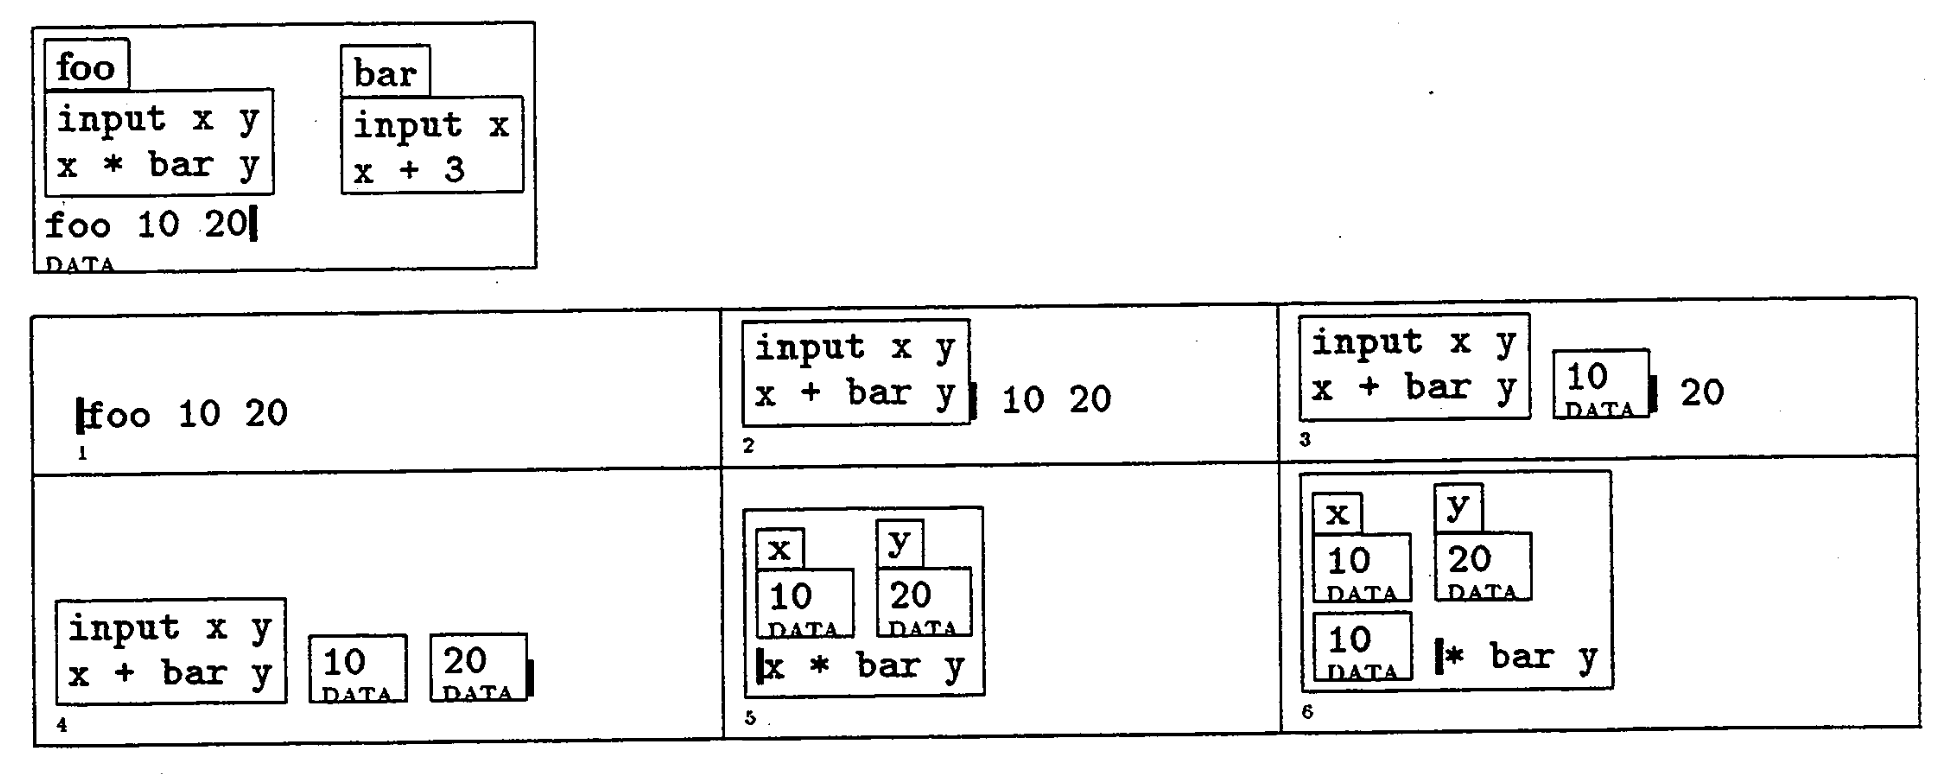
\includegraphics[width=0.9\linewidth]{fig/stepper.png}
\caption{First six step of the execution of \texttt{foo 10 20} in the Boxer movie stepper.
  The box above shows the original source code. The box below shows the successive steps.
  (1) The evaluation starts, (2) function definition repalces the
  reference, (3, 4) arguments are wrapped in data boxes, (5) \texttt{input} is replaced with
  boxes passed as arguments and (6) \texttt{x} is replaced with the variable value.
  (Image source~\cite{klotz-1989-boxer})}
\label{fig:stepper}
\end{figure}

\paragraph{Example: Boxer.}
The evaluation model of Boxer~\cite{disessa-1986-boxer} is based on the idea of \emph{copying
semantics}. In this model, the evaluation of a reference to another box proceeds by replacing
the reference with the box itself. The user does not see this during normal use of the system, but
the Boxer movie stepper \cite{klotz-1989-boxer} makes it possible to see how the exeuction
proceeds step-by-step. As illustrated in Figure~\ref{fig:stepper}, the execution can be seen as
a sequence of (mutable) transformations of the document.

\subsection{Identification of Nodes}
\label{sec:eval-ident}
When manipulating documents, the document-oriented programming system (and code that it runs)
needs some mechanism for referring to other elements in the document. There are multiple approaches
and a programming system may support a combination of these.

\begin{itemize}
\item \emph{Human-Readable Identifiers.}
  The most common approach is to let users name elements they want to refer to using a variable
  name or human-readable identifier for a document element
  (Jupyter~\cite{kluyver-2016-jupyter}, HyperCard~\cite{atkinson-1987-hypercard},
  Boxer~\cite{disessa-1986-boxer}, Webstrates~\cite{klokmose-2015-webstrates}).
  Names are typically global, although a system could also support namespaces.

\item \emph{Absolute Paths.}
  In systems with a richer document structure, elements can be referred to by a
  pre-defined addressing scheme (Spreadsheets~\cite{abraham-2009-spreadsheets}) or by
  using a path (a sequence of node names) from the root (Denicek~\cite{petricek-2025-denicek},
  HyperCard~\cite{atkinson-1987-hypercard}). In HyperCard, elements on different cards can have
  the same name and one refers to them using a path consisting of the stack name, card name
  and an element name.

\item \emph{Internal Unique Identifiers.}
  To sidestep fragile named references, some programming systems use internal unique identifiers,
  not visible to the user. The user may see a name, a visual representation of the reference
  or the referenced value, directly in place of the reference
  (Subtext~\cite{edwards-2005-subtext}). Note that maintaining internal unique identifiers
  typically requires using a structure editor.

\item \emph{Relative References.}
  In addition to other mechanisms, document nodes can refer to document other nodes through paths
  that are relative to their location in the document
  (Spreadsheets \cite{abraham-2009-spreadsheets}, Denicek \cite{petricek-2025-denicek}).
  In trees, this typically requires the ability to refer to a parent element. In spreadsheets
  dollar references (e.g., \texttt{\$B\$10}) are absolute and ordinary references (e.g., \texttt{B10})
  are relative.

\item \emph{Selectors.}
  A richer referencing mechanism allows the user to specify nodes using a combination of
  paths and selectors, for example to refer to all children of a node, children of a specific
  tag or class (as in CSS selectors), or an element of a given shape anywhere in the document
  (Webstrates~\cite{klokmose-2015-webstrates}, Denicek \cite{petricek-2025-denicek}).
\end{itemize}

\paragraph{Example: Denicek and Subtext.}
Identification of nodes poses an interesting problem in systems where document nodes can be
moved and renamed, or in systems based on edit histories (see \S\ref{sec:struct-repr})
where edits need to be merged or reconcilled. Two systems that tackle this problem are
Subtext~\cite{edwards-2005-subtext} and Denicek \cite{petricek-2025-denicek}.

For example, say we have a document with a root node named \texttt{pioneers} containing two
children named \texttt{lovelace} and \texttt{hamilton}. In Denicek, one can refer to a
specific node using an \emph{Absolute Path} such as \texttt{/pioneers/lovelace} or to multiple
nodes using a \emph{Selector} \texttt{/pioneers/*}. Subtext, by contrast, uses \emph{Internal Unique
Identifiers} and the selection made by the user results in a collection of IDs, referring to
the selected nodes.

The first consequence of the design choice is how the systems handle renaming of nodes.
In Subtext, renaming \texttt{pioneers} to \texttt{compsci} has no effect on the unique
identifiers. In Denicek, the operation requires updating all references, for example, from
\texttt{/pioneers/*} to~\texttt{/compsci/*}.

The design choice has interesting consequences when merging edits. If a user makes edit using
a selector (such as \texttt{/pioneers/*}) in a system identifies nodes through \emph{Selectors},
the edit affects all nodes including those that may have been created independently and have been
merged with the current document (a scenario illustrated in \cite{edwards-2024-schema}).
When the system identifies nodes through \emph{Internal Unique Identifiers}, only nodes known
when the edit was done will be affected. On the other hand, merging of edits is challenging when
the system uses expressive language of selectors (and Denicek restricts the expressivity of
selectors to make merging tractable \cite{petricek-2025-denicek}).

\newpage
% TODO: Where to put Forms/3 - ask Jonathan
% https://web.archive.org/web/20220120223923/http://cajun.cs.nott.ac.uk/compsci/epo/papers/volume7/issue2/ep078vq.pdf

\cite{petricek-2018-wrattler}
\cite{kluyver-2016-jupyter}
forms/3 \cite{burnett-2001-forms3}

Lopecode~\cite{larkworthy-2025-lopecodetour}

spreadsheets \cite{abraham-2009-spreadsheets}
subtext \cite{edwards-2005-subtext}
denicek \cite{petricek-2025-denicek}
hypercard \cite{atkinson-1987-hypercard}
jupyter \cite{kluyver-2016-jupyter}
c.f. wrattler more live
boxer \cite{disessa-1986-boxer}

ampleforth \cite{bracha-2022-ampleforth,bracha-2024-docuapps}
bootrstraplab \cite{jakubovic-2022-bootstraplab}
hazel \cite{omar-2021-livelits} \cite{omar-2017-hazelnut}
webstrates \cite{klokmose-2015-webstrates}

potluck \cite{litt-2022-potluck}
%embark \cite{sonnentag-2023-embark}

ampleforth can be anything




---

\cite{ohshima-2025-renkonpad} -- maybe not exactly document but around DOM

Videostrates https://pure.au.dk/ws/portalfiles/portal/164699070/VideostratesUIST2019.pdf
are docs with videos

Active \cite{quint-1994-active}
EmbeddedButtons \cite{bier-1991-docs,bier-1991-buttons}


spreadsheets\cite{abraham-2009-spreadsheets}
subtext \cite{edwards-2005-subtext}
hypercard \cite{atkinson-1987-hypercard}
jupyter \cite{kluyver-2016-jupyter}
c.f. wrattler more live
boxer \cite{disessa-1986-boxer}

ampleforth \cite{bracha-2022-ampleforth,bracha-2024-docuapps}
hazel \cite{omar-2021-livelits} \cite{omar-2017-hazelnut}
bootrstraplab \cite{jakubovic-2022-bootstraplab}
denicek \cite{petricek-2025-denicek}
webstrates \cite{klokmose-2015-webstrates}

potluck \cite{litt-2022-potluck}
%embark \cite{sonnentag-2023-embark}

\section{Related work}
not about programming sytems \cite{crichton-2024-document}
json editor, but similar to livelits \cite{mcnutt-2023-projectional}
Self - not quite documents, but objects as UI

antranig's thing - maybe
Varv - maybe

transclusion - used in ampleforth

c.f. Rein's literature review - but it is more difficult to google this

\newpage

\bibliography{paper}
\end{document}

% Local Variables:
% TeX-engine: luatex
% End:
